\documentclass[tikz,border=8pt]{standalone}
\usepackage[T1]{fontenc}
\usepackage{inter}
\renewcommand{\familydefault}{\sfdefault}
\usepackage{amsmath,amssymb}
\usetikzlibrary{arrows.meta,calc,decorations.pathreplacing,positioning,backgrounds}

% palette
\definecolor{readc}{RGB}{27,127,107}
\definecolor{writec}{RGB}{47,85,201}
\definecolor{mapc}{RGB}{31,108,128}
\definecolor{blk}{RGB}{232,232,232}
\definecolor{blkb}{RGB}{160,160,160}
\definecolor{txt}{RGB}{60,60,60}
\definecolor{note}{RGB}{110,110,110}
\definecolor{panel}{RGB}{245,245,245}

\tikzset{
  blk/.style={draw=blkb,fill=blk,rounded corners=1.2pt,minimum width=0.50cm,minimum height=0.28cm,inner sep=0pt,line width=0.4pt},
  up/.style={-{Stealth[length=1.3mm,width=1.1mm]},blkb,line width=0.45pt},
  dots/.style={blkb,line width=0.45pt,dotted},
  lab/.style={font=\small,text=txt},
  small/.style={font=\scriptsize,text=note},
  tok/.style={font=\ttfamily\small,text=txt,rotate=90,anchor=east},
  marker/.style={circle,inner sep=0pt,minimum size=0.36cm,text=white,font=\bfseries\scriptsize},
  attn/.style={-{Stealth[length=1.6mm,width=1.4mm]},line width=0.7pt},
  halo/.style={white,line width=2.4pt},
  flow/.style={-{Stealth[length=1.6mm,width=1.4mm]},line width=0.8pt},
}

% \vstack{name}{x}{y}{base colour}{shade list (4 entries, % of base)}
\newcommand{\vstack}[5]{%
  \begin{scope}[shift={(#2,#3)}]
    \foreach \s [count=\k] in {#5}{%
      \fill[#4!\s!white,draw=white,line width=0.3pt] (-0.15,{0.46-0.23*\k}) rectangle (0.15,{0.46-0.23*(\k-1)});
    }
    \draw[#4!60!black,line width=0.35pt,rounded corners=0.6pt] (-0.15,-0.46) rectangle (0.15,0.46);
    \coordinate (#1) at (0,0);
    \coordinate (#1-n) at (0,0.46);
    \coordinate (#1-s) at (0,-0.46);
    \coordinate (#1-e) at (0.15,0);
    \coordinate (#1-w) at (-0.15,0);
  \end{scope}}

% big vector stack for right side: 5 cells
\newcommand{\bstack}[5]{%
  \begin{scope}[shift={(#2,#3)}]
    \foreach \s [count=\k] in {#5}{%
      \fill[#4!\s!white,draw=white,line width=0.4pt] (-0.19,{0.7-0.28*\k}) rectangle (0.19,{0.7-0.28*(\k-1)});
    }
    \draw[#4!60!black,line width=0.4pt,rounded corners=0.8pt] (-0.19,-0.7) rectangle (0.19,0.7);
    \coordinate (#1) at (0,0);
    \coordinate (#1-n) at (0,0.7);
    \coordinate (#1-s) at (0,-0.7);
    \coordinate (#1-e) at (0.19,0);
    \coordinate (#1-w) at (-0.19,0);
  \end{scope}}

\begin{document}
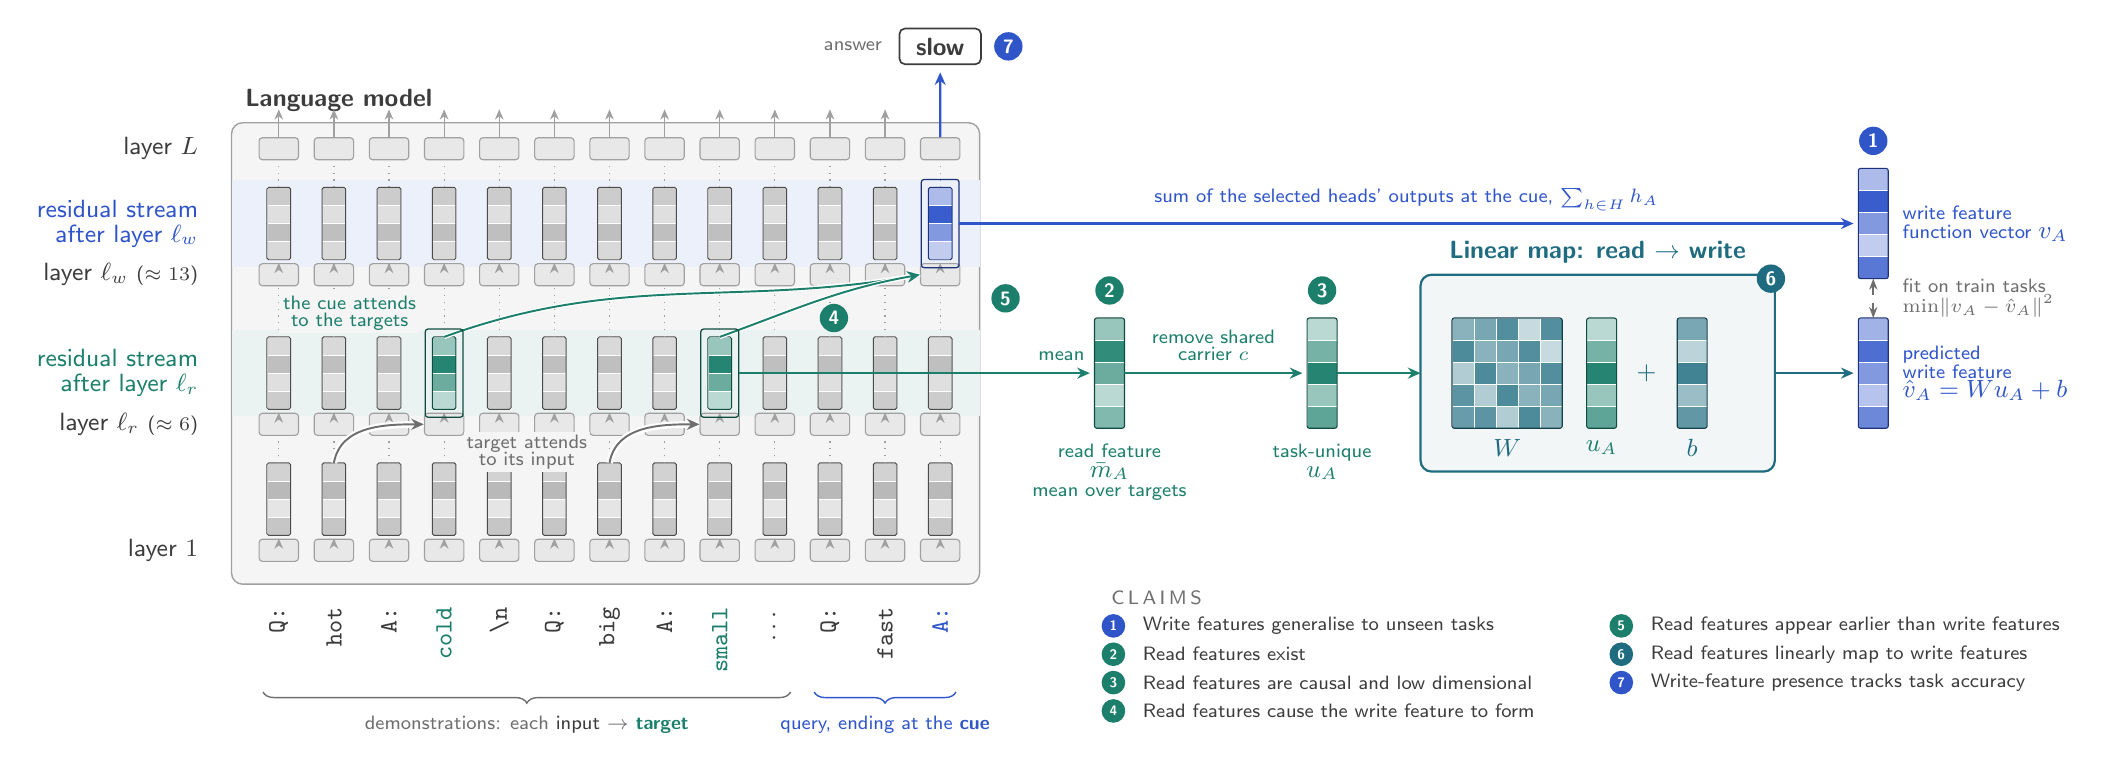
\begin{tikzpicture}[x=1cm,y=1cm]

% ---------------- geometry ----------------
\def\dx{0.70}
\def\xo{0.85}
\def\yLone{0.55}    % layer 1 block
\def\yRone{1.20}    % residual after layer 1
\def\yLr{2.15}      % read layer block
\def\yRr{2.80}      % residual after read layer
\def\yLw{4.05}      % write layer block
\def\yRw{4.70}      % residual after write layer
\def\yLL{5.65}      % layer L block
\def\yTop{6.15}

% LM panel
\begin{scope}[on background layer]
  \fill[panel,draw=blkb,rounded corners=4pt,line width=0.5pt] (0.25,0.12) rectangle (9.75,5.98);
  \fill[readc!9!white] (0.25,\yRr-0.55) rectangle (9.75,\yRr+0.55);
  \fill[writec!9!white] (0.25,\yRw-0.55) rectangle (9.75,\yRw+0.55);
\end{scope}
\node[lab,font=\small\bfseries,anchor=south west] at (0.3,6.0) {Language model};

% columns
\foreach \tk/\role [count=\i] in {Q:/o, hot/i, A:/o, cold/t, {\char`\\n}/o, Q:/o, big/i, A:/o, small/t, {$\cdots$}/d, Q:/o, fast/i, A:/c}{
  \pgfmathsetmacro{\x}{\xo+\dx*(\i-1)}
  \coordinate (c\i) at (\x,0);
  % layer 1
  \node[blk] (b1-\i) at (\x,\yLone) {};
  \draw[up] (b1-\i.north) -- (\x,\yRone-0.5);
  \vstack{r1-\i}{\x}{\yRone}{gray}{35,55,20,45}
  \draw[dots] (r1-\i-n) -- (\x,\yLr-0.16);
  % read layer
  \node[blk] (br-\i) at (\x,\yLr) {};
  \draw[up] (br-\i.north) -- (\x,\yRr-0.5);
  \if\role t
    \vstack{rr-\i}{\x}{\yRr}{readc}{45,95,65,30}
  \else
    \vstack{rr-\i}{\x}{\yRr}{gray}{30,50,25,40}
  \fi
  \draw[dots] (rr-\i-n) -- (\x,\yLw-0.16);
  % write layer
  \node[blk] (bw-\i) at (\x,\yLw) {};
  \draw[up] (bw-\i.north) -- (\x,\yRw-0.5);
  \if\role c
    \vstack{rw-\i}{\x}{\yRw}{writec}{40,95,60,30}
  \else
    \vstack{rw-\i}{\x}{\yRw}{gray}{40,25,50,30}
  \fi
  \draw[dots] (rw-\i-n) -- (\x,\yLL-0.16);
  % layer L
  \node[blk] (bL-\i) at (\x,\yLL) {};
  \if\role c\else \draw[up] (bL-\i.north) -- (\x,\yTop); \fi
  % token label
  \if\role t \node[tok,text=readc,font=\ttfamily\small\bfseries] at (\x,-0.05) {\tk};
  \else\if\role c \node[tok,text=writec,font=\ttfamily\small\bfseries] at (\x,-0.05) {\tk};
  \else \node[tok] at (\x,-0.05) {\tk};
  \fi\fi
}

% cue -> answer
\draw[flow,writec] (bL-13.north) -- (9.25,6.62);
\node[draw=txt,fill=white,rounded corners=2pt,line width=0.6pt,font=\small\bfseries,text=txt,minimum height=0.44cm,inner xsep=6pt] (ans) at (9.25,6.95) {slow};
\node[small,anchor=east] at (ans.west) {answer\ \ };
\node[marker,fill=writec,anchor=west] at ($(ans.east)+(0.15,0)$) {7};

% left labels
\node[lab,anchor=east] at (-0.05,\yLone) {layer $1$};
\node[lab,anchor=east] at (-0.05,\yLr) {layer $\ell_{r}$ {\scriptsize($\approx 6$)}};
\node[lab,anchor=east,align=right,text=readc] at (-0.05,\yRr) {residual stream\\[-2pt]after layer $\ell_{r}$};
\node[lab,anchor=east] at (-0.05,\yLw) {layer $\ell_{w}$ {\scriptsize($\approx 13$)}};
\node[lab,anchor=east,align=right,text=writec] at (-0.05,\yRw) {residual stream\\[-2pt]after layer $\ell_{w}$};
\node[lab,anchor=east] at (-0.05,\yLL) {layer $L$};
\node[marker,fill=readc] at (10.08,{(\yRr+\yRw)/2}) {5};

% token-role labels + braces
\pgfmathsetmacro{\xa}{\xo}
\pgfmathsetmacro{\xb}{\xo+\dx*9}
\pgfmathsetmacro{\xc}{\xo+\dx*10}
\pgfmathsetmacro{\xd}{\xo+\dx*12}
\draw[decorate,decoration={brace,mirror,amplitude=4pt},note,line width=0.5pt] (\xa-0.2,-1.25) -- (\xb+0.2,-1.25)
  node[midway,below=5pt,small] {demonstrations: each \textcolor{txt}{input} $\rightarrow$ \textcolor{readc}{\textbf{target}}};
\draw[decorate,decoration={brace,mirror,amplitude=4pt},writec,line width=0.5pt] (\xc-0.2,-1.25) -- (\xd+0.2,-1.25)
  node[midway,below=5pt,small,text=writec] {query, ending at the \textbf{cue}};

% ---------------- attention arcs ----------------
% target attends to its input (early)
\foreach \a/\b in {2/4, 7/9}{
  \draw[halo] (r1-\a-n) to[out=80,in=180] (br-\b.west);
  \draw[attn,note] (r1-\a-n) to[out=80,in=180] (br-\b.west);
}
\node[small,fill=panel,inner sep=1pt,align=center] at ($(c5)+(0.35,1.80)$) {target attends\\[-2pt]to its input};
% cue attends to the targets (mid)
\foreach \a in {4,9}{
  \draw[halo,line width=1.6pt] (rr-\a-n) to[out=20,in=190] (bw-13.west);
  \draw[attn,readc] (rr-\a-n) to[out=20,in=190] (bw-13.west);
}
\node[small,fill=panel,inner sep=1pt,text=readc,align=center] at ($(c2)+(0.20,3.56)$) {the cue attends\\[-2pt]to the targets};
\node[marker,fill=readc] at ($(c11)+(0.05,3.50)$) {4};

% ---------------- right side: read feature ----------------
\draw[readc!60!black,line width=0.45pt,rounded corners=1pt] ($(rr-4)+(-0.24,-0.56)$) rectangle ($(rr-4)+(0.24,0.56)$);
\draw[readc!60!black,line width=0.45pt,rounded corners=1pt] ($(rr-9)+(-0.24,-0.56)$) rectangle ($(rr-9)+(0.24,0.56)$);
\draw[flow,readc] ($(rr-9)+(0.24,0)$) -- ++(0.18,0) -- (10.55,\yRr) -- (11.15,\yRr)
  node[pos=0.40,above=1pt,small,text=readc] {mean};
\bstack{mA}{11.40}{\yRr}{readc}{45,90,65,30,55}
\node[small,align=center,text=readc,anchor=north] at (11.40,\yRr-0.78) {read feature\\[-1pt]{\small $\bar m_A$}\\[-1pt]mean over targets};
\node[marker,fill=readc] at (11.40,\yRr+1.05) {2};

\draw[flow,readc] (mA-e) -- (13.85,\yRr)
  node[midway,above=1pt,small,text=readc,align=center] {remove shared\\[-2pt]carrier $c$};
\bstack{uA}{14.10}{\yRr}{readc}{30,60,95,45,70}
\node[small,align=center,text=readc,anchor=north] at (14.10,\yRr-0.78) {task-unique\\[-1pt]{\small $u_A$}};
\node[marker,fill=readc] at (14.10,\yRr+1.05) {3};

% ---------------- linear map box ----------------
\def\bxl{15.35}\def\bxr{19.85}\def\byb{1.55}\def\byt{4.05}
\draw[mapc,fill=mapc!6!white,rounded corners=4pt,line width=0.8pt] (\bxl,\byb) rectangle (\bxr,\byt);
\node[font=\small\bfseries,text=mapc,anchor=south] at ({(\bxl+\bxr)/2},\byt+0.02) {Linear map: read $\rightarrow$ write};
\draw[flow,readc] (uA-e) -- (\bxl,\yRr);
% matrix W
\begin{scope}[shift={(16.45,\yRr)}]
  \foreach \i in {0,...,4}{\foreach \j in {0,...,4}{
    \pgfmathsetmacro{\sh}{25+55*abs(sin(70*\i+110*\j+30))}
    \fill[mapc!\sh!white,draw=white,line width=0.4pt] ({-0.7+0.28*\j},{0.7-0.28*(\i+1)}) rectangle ({-0.7+0.28*(\j+1)},{0.7-0.28*\i});
  }}
  \draw[mapc!60!black,line width=0.4pt,rounded corners=0.8pt] (-0.7,-0.7) rectangle (0.7,0.7);
\end{scope}
\node[small,text=mapc] at (16.45,\yRr-0.95) {\small $W$};
\bstack{uAin}{17.65}{\yRr}{readc}{30,60,95,45,70}
\node[small,text=readc] at (17.65,\yRr-0.95) {\small $u_A$};
\node[lab,text=mapc] at (18.22,\yRr) {$+$};
\bstack{bvec}{18.80}{\yRr}{mapc}{60,30,85,45,70}
\node[small,text=mapc] at (18.80,\yRr-0.95) {\small $b$};
\node[marker,fill=mapc] at (\bxr-0.05,\byt-0.05) {6};

% prediction
\draw[flow,mapc] (\bxr,\yRr) -- (20.85,\yRr);
\bstack{vhat}{21.10}{\yRr}{writec}{45,85,60,35,70}
\node[small,align=left,anchor=west,text=writec] at (21.35,\yRr) {predicted\\[-1pt]write feature\\[-1pt]{\small $\hat v_A = W u_A + b$}};

% ---------------- right side: write feature ----------------
\draw[writec!60!black,line width=0.45pt,rounded corners=1pt] ($(rw-13)+(-0.24,-0.56)$) rectangle ($(rw-13)+(0.24,0.56)$);
\draw[flow,writec] ($(rw-13)+(0.24,0)$) -- (20.85,\yRw)
  node[pos=0.50,above=1pt,small,text=writec,align=center] {sum of the selected heads' outputs at the cue, $\sum_{h\in H} h_A$};
\bstack{vA}{21.10}{\yRw}{writec}{40,95,60,30,80}
\node[small,align=left,anchor=west,text=writec] at (21.35,\yRw) {write feature\\[-1pt]function vector {\small $v_A$}};
\node[marker,fill=writec] at (21.10,\yRw+1.05) {1};

% fit
\draw[{Stealth[length=1.4mm]}-{Stealth[length=1.4mm]},note,dashed,line width=0.6pt] (vhat-n) -- (vA-s);
\node[small,anchor=west,align=left] at (21.35,{(\yRr+\yRw)/2}) {fit on train tasks\\[-1pt]$\min \lVert v_A - \hat v_A\rVert^2$};

% ---------------- claims legend ----------------
\begin{scope}[shift={(11.3,-0.05)}]
  \node[font=\scriptsize,text=note,anchor=west] at (0,0) {C\,L\,A\,I\,M\,S};
  \foreach \n/\col/\t [count=\k] in {
     1/writec/{Write features generalise to unseen tasks},
     2/readc/{Read features exist},
     3/readc/{Read features are causal and low dimensional},
     4/readc/{Read features cause the write feature to form}}{
    \node[marker,fill=\col,minimum size=0.30cm,font=\bfseries\tiny] at (0.15,{-0.36*\k}) {\n};
    \node[small,anchor=west,text=txt] at (0.40,{-0.36*\k}) {\t};
  }
  \foreach \n/\col/\t [count=\k] in {
     5/readc/{Read features appear earlier than write features},
     6/mapc/{Read features linearly map to write features},
     7/writec/{Write-feature presence tracks task accuracy}}{
    \node[marker,fill=\col,minimum size=0.30cm,font=\bfseries\tiny] at (6.6,{-0.36*\k}) {\n};
    \node[small,anchor=west,text=txt] at (6.85,{-0.36*\k}) {\t};
  }
\end{scope}

\end{tikzpicture}
\end{document}
